\documentclass{article}

\PassOptionsToPackage{numbers,compress}{natbib}
\PassOptionsToPackage{hypertexnames=false}{hyperref}
\usepackage[eandd,preprint]{neurips_2026}

\usepackage[utf8]{inputenc}
\usepackage[T1]{fontenc}
\usepackage{hyperref}
\usepackage{url}
\usepackage{booktabs}
\usepackage{amsmath}
\usepackage{amssymb}
\usepackage{microtype}
\usepackage{xcolor}
\usepackage{graphicx}
\usepackage{float}
\usepackage{enumitem}
\usepackage{placeins}

\setlist[itemize]{itemsep=1pt, topsep=2pt, parsep=0pt, partopsep=0pt}
\setlength{\abovecaptionskip}{4pt}
\setlength{\belowcaptionskip}{2pt}
\graphicspath{{figures/}{figures/supp/}}

\newcommand{\fcsc}{FC$\rightarrow$SC}
\newcommand{\scfc}{SC$\rightarrow$FC}
\newcommand{\dpear}{\texttt{demeaned\_pearson}}
\newcommand{\bvdemo}{\texttt{bv+demo}}

% number supplementary figures/tables with an S prefix
\renewcommand{\thefigure}{S\arabic{figure}}
\renewcommand{\thetable}{S\arabic{table}}
\renewcommand{\thesection}{S\arabic{section}}

\title{Supplementary Material --- Sanity Checks and Reproducibility\\
\large What Cross-Modal Connectome Prediction Does and Does Not Buy}

\author{%
  Adel Sahuc \\
  New York University Tandon School of Engineering \\
  \texttt{ans9868@nyu.edu}%
}

\begin{document}
\maketitle

\noindent
This supplement documents, in full, the sanity-check discipline behind the main paper. The
purpose is not to pad the results with extra numbers but to show that each headline claim was
actively attacked from the directions a skeptical reviewer would choose, and survived. Every
section corresponds to a self-contained check in the project tree; the source artifacts are
named at the end of each section, and all values are reproduced from the committed CSV / findings
outputs of those checks.

\paragraph{The three claims under test.}
\begin{enumerate}
\item \textbf{Directional reconstruction.} FC predicts SC better than SC predicts FC
($\approx 1.6$--$1.7\times$ in \dpear), stable across seeds and parcellations.
\item \textbf{No automatic utility.} A cheap \bvdemo{} baseline predicts cognition; only
observed FC beats it; observed SC and imputed connectomes do not, and \texttt{pred\_FC} is
actively harmful.
\item \textbf{Objective-dependent identity signal.} Predicted SC carries heritable family
signal, but only under objectives that preserve it.
\end{enumerate}

\paragraph{Index of checks.}
\begin{table}[h]
\centering\small
\begin{tabular}{@{}cl l l@{}}
\toprule
\textbf{\S} & \textbf{Check} & \textbf{Attacks the explanation} & \textbf{Verdict} \\
\midrule
S1 & Reduction-axis robustness & ``the asymmetry is a PCA artifact'' & closed \\
S2 & FC noise \& reliability ceilings & ``\scfc{} fails because FC is noisy'' & closed (FC-side) \\
S3 & Nonlinear model class & ``a bigger/nonlinear model would find it'' & closed \\
S4 & Residual-boost \& multimodal sink & ``the linear model left signal on the table'' & closed \\
S5 & Sample-size scaling & ``more subjects would unlock it'' & closed ($n\!\approx\!683$) \\
S6 & Richer structural representation & ``streamline counts are too crude'' & closed \\
S7 & PC mechanism localization & ``the family mode is a reliability artifact'' & survives \\
S8 & Completeness, leaks, reproducibility & ``the grid is silently wrong'' & clean \\
\bottomrule
\end{tabular}
\end{table}

\paragraph{Two ceilings.} A recurring distinction runs through several sections.
\emph{Ceiling A} (data reproducibility) is how well the target agrees with a repeat
measurement of itself; it bounds recoverable biological signal but is valid only at the
population level. \emph{Ceiling B} (model/oracle) is how well the same estimator predicts the
target from a perfect same-modality copy (\mbox{FC$\rightarrow$FC}, \mbox{SC$\rightarrow$SC});
it is available for both modalities and never exceeded per subject, but is looser because it
can exploit session-specific signal that would not replicate. We disattenuate biological
claims against Ceiling A and use Ceiling B only to quantify cross-modal-vs-within-modality loss.

\FloatBarrier
\section{Reduction-Axis Robustness}

\textbf{Concern.} The headline \fcsc{} $>$ \scfc{} asymmetry was computed with one pipeline
(PCA(256) source, PLS(64) latents, inverse-PCA target). Is the asymmetry a property of the
brain or of that learned reduction?

\textbf{Design.} A three-point ladder over 10 seeds, both directions: (A) PCA$\rightarrow$PLS
$\rightarrow$PCA (main); (B) full PLS on the raw 64{,}620-edge vectors (no reduction); (C)
input PCA replaced by data-blind Johnson--Lindenstrauss random projections (Gaussian dense,
sparse $\approx 1/\sqrt{p}$, sparse $1/3$). If A, B, C agree, the reduction is neither hiding
nor injecting the effect.

\begin{table}[h]
\centering\small
\caption{All five reduction strategies preserve \fcsc{} $>$ \scfc{} at Wilcoxon $p\le 0.001$.}
\begin{tabular}{@{}lrrrrrr@{}}
\toprule
\textbf{Method (n=10)} & \textbf{med \fcsc} & \textbf{med \scfc} & \textbf{med ratio} & \textbf{min} & \textbf{max} & \textbf{p vs 1} \\
\midrule
PCA$\rightarrow$PLS$\rightarrow$PCA (main) & 0.1355 & 0.0847 & \textbf{1.621$\times$} & 1.32 & 1.86 & 0.001 \\
Full PLS (raw 64{,}620-dim) & 0.1382 & 0.0762 & \textbf{1.813$\times$} & 1.49 & 2.11 & 0.001 \\
JL Gaussian dense & 0.0837 & 0.0610 & \textbf{1.397$\times$} & 1.19 & 2.25 & 0.001 \\
JL sparse-auto ($\approx 1/\sqrt{p}$) & 0.0841 & 0.0592 & \textbf{1.389$\times$} & 1.11 & 1.90 & 0.001 \\
JL sparse-1/3 (Achlioptas) & 0.0846 & 0.0535 & \textbf{1.554$\times$} & 1.24 & 1.78 & 0.001 \\
\bottomrule
\end{tabular}
\end{table}

\textbf{Reading.} Full PLS ($1.81\times$) $\ge$ baseline ($1.62\times$): removing reduction
entirely gives the same direction and a slightly stronger magnitude, so PCA modestly
\emph{attenuates} rather than creates the asymmetry. The JL variants ($1.39$--$1.55\times$)
lower the absolute \dpear{} (they lose PCA's variance concentration) but preserve the ratio.
The magnitude spread is wider than $\pm 0.15\times$ but lies between known-equivalent
reductions; the direction is unambiguous.

\begin{figure}[h]
  \centering
  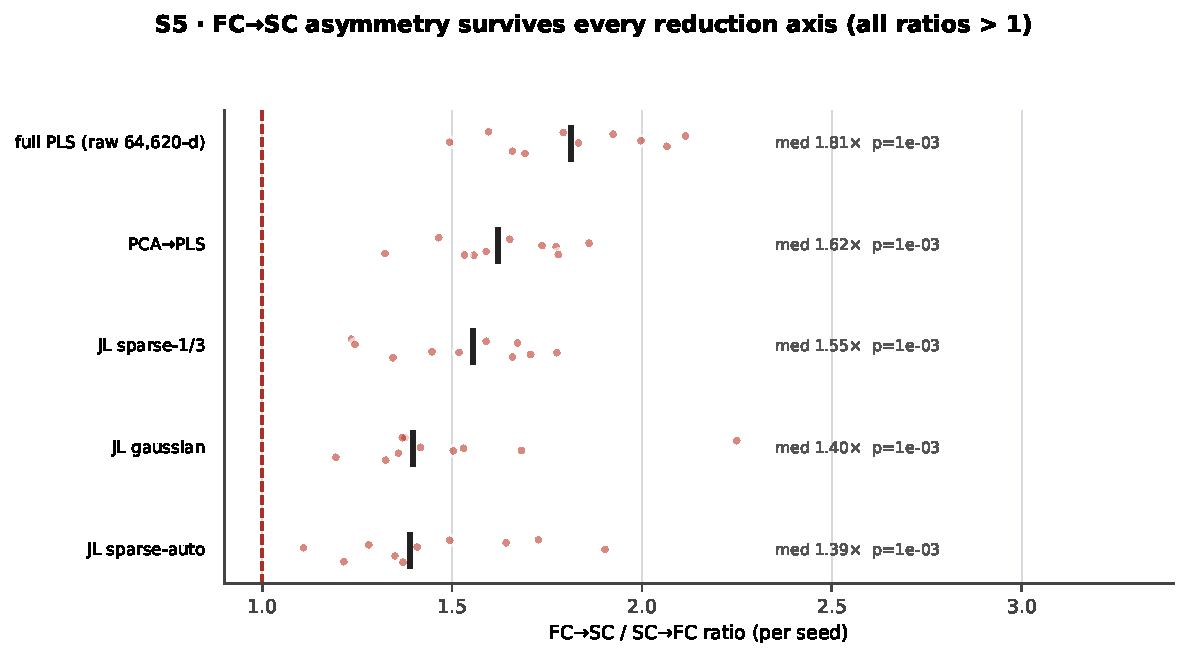
\includegraphics[width=0.78\linewidth]{S5_reduction_axis.pdf}
  \caption{Per-seed \fcsc{}/\scfc{} ratios for all five reduction strategies; every ratio
  exceeds 1, all Wilcoxon $p\le 0.001$.}
\end{figure}

\noindent\emph{Source:} \texttt{sanity\_checks/preprocessing\_check/}.

\FloatBarrier
\section{FC Measurement Noise and Reliability Ceilings}

\textbf{Concern.} \scfc{} is weak --- perhaps only because FC is a noisy target, not because
SC and FC are genuinely independent.

\textbf{FC is mostly edge-noise but reliable as a whole connectome.}

\begin{table}[h]
\centering\small
\caption{Variance decomposition of single-edge FC (individual-difference fractions sum to 1).}
\begin{tabular}{@{}lrrrrr@{}}
\toprule
\textbf{Parcellation} & \textbf{trait} & \textbf{state (day)} & \textbf{within-session} & \textbf{noise} & \textbf{G (avg)} \\
\midrule
Glasser & 0.301 & 0.035 & 0.021 & \textbf{0.643} & 0.585 \\
4S456Parcels & 0.261 & 0.035 & 0.021 & \textbf{0.683} & 0.519 \\
\bottomrule
\end{tabular}
\end{table}

At the single-edge level $\sim$64--68\% of between-subject variance is noise, yet the whole
connectome is 93\% identifiable (fingerprint top1 0.927 / 0.934; discriminability $\approx
0.998$). Individual signal is \emph{distributed}: each edge is noisy, the multivariate pattern
is stable.

\begin{table}[h]
\centering\small
\caption{FC reliability ceiling. The valid ceiling is between-session (0.491 Glasser); the
within-session rung is lower due to the LR/RL phase-encode distortion confound.}
\begin{tabular}{@{}llrrrr@{}}
\toprule
\textbf{Parc} & \textbf{comparison} & \textbf{demeaned\_r} & \textbf{pearson} & \textbf{top1} & \textbf{avg\_rank} \\
\midrule
Glasser & within-session (LR/RL) & 0.364 & 0.710 & 0.78 & 0.968 \\
Glasser & \textbf{between-session (REST1/REST2)} & \textbf{0.491} & 0.813 & 0.933 & 0.992 \\
4S456 & within-session (LR/RL) & 0.337 & 0.670 & 0.78 & 0.969 \\
4S456 & between-session (REST1/REST2) & 0.457 & 0.783 & 0.936 & 0.993 \\
\bottomrule
\end{tabular}
\end{table}

\begin{table}[h]
\centering\small
\caption{Cross-modal disattenuation against the FC reproducibility ceiling (0.491).
\scfc{} captures only $\sim$17\% of reproducible FC.}
\begin{tabular}{@{}llrrr@{}}
\toprule
\textbf{source $\rightarrow$ FC} & \textbf{metric} & \textbf{achieved} & \textbf{ceiling} & \textbf{fraction} \\
\midrule
\textbf{\scfc} & demeaned\_r & 0.085 & 0.491 & \textbf{0.17} \\
\scfc & top1 (fingerprint) & 0.051 & 0.933 & 0.05 \\
\scfc & avg\_rank & 0.713 & 0.992 & 0.72 \\
\bvdemo$\rightarrow$FC & demeaned\_r & 0.098 & 0.491 & 0.20 \\
\bvdemo$\rightarrow$FC & top1 & 0.026 & 0.933 & 0.03 \\
\bottomrule
\end{tabular}
\end{table}

\textbf{Per-subject reliability does not explain \scfc.} Per-subject FC reliability is
heterogeneous (mean 0.489, range $\approx 0$--$0.78$) and a stable trait (within-vs-between
$\rho=0.41$). A subject's \scfc{} quality is \emph{uncorrelated} with their FC reliability
(Pearson $r=0.01$, $p=0.72$), whereas \bvdemo$\rightarrow$FC weakly tracks it ($r=0.15$),
proving the test can detect a reliability effect when one exists. Reliability-filtering makes
the captured fraction \emph{worse} (raising the ceiling 0.49$\to$0.58 while achieved stays
pinned at $\sim$0.08). The shortfall is decisively not an FC-noise or per-subject-reliability
artifact; the only open piece is SC's own reliability (data-blocked: no test-retest dMRI in
HCP-YA).

\begin{figure}[h]
  \centering
  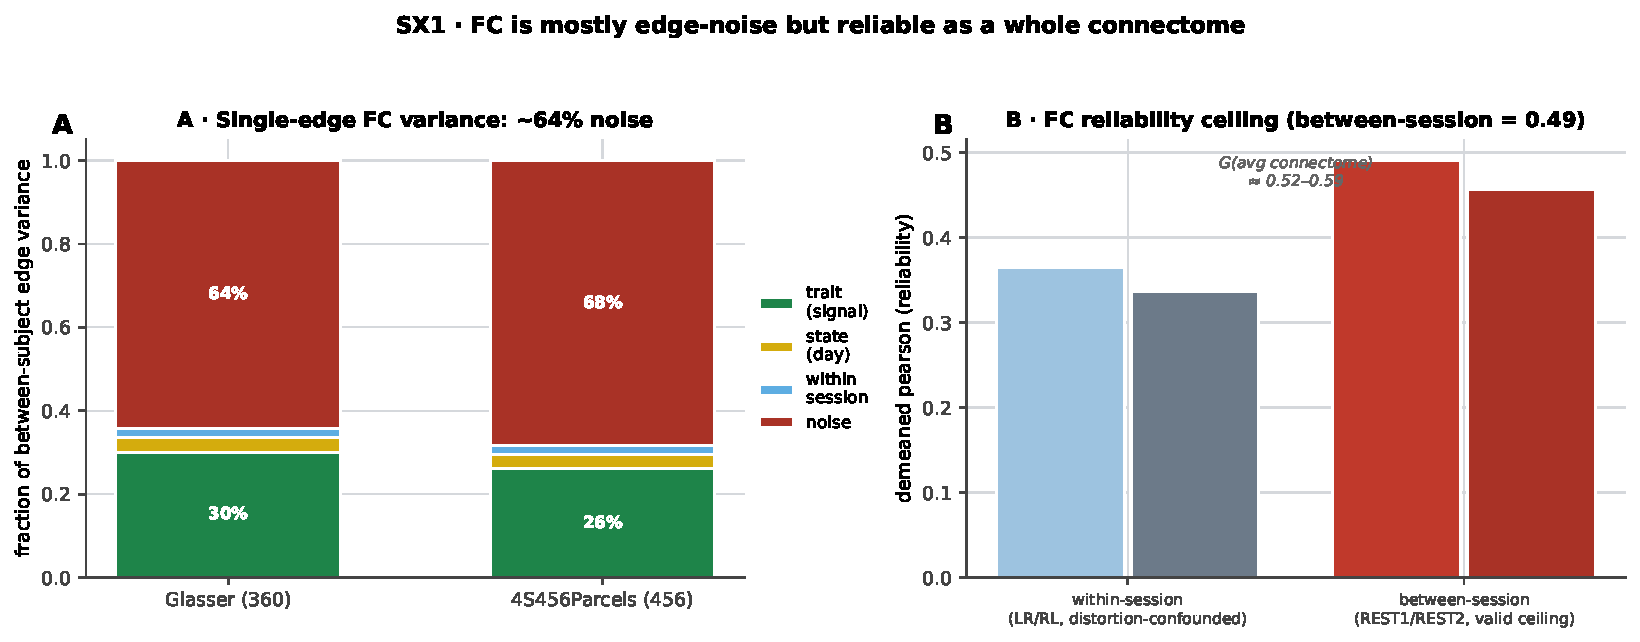
\includegraphics[width=\linewidth]{SX1_variance_reliability.pdf}
  \caption{FC variance decomposition (left) and reliability-ceiling rungs (right).}
\end{figure}
\begin{figure}[h]
  \centering
  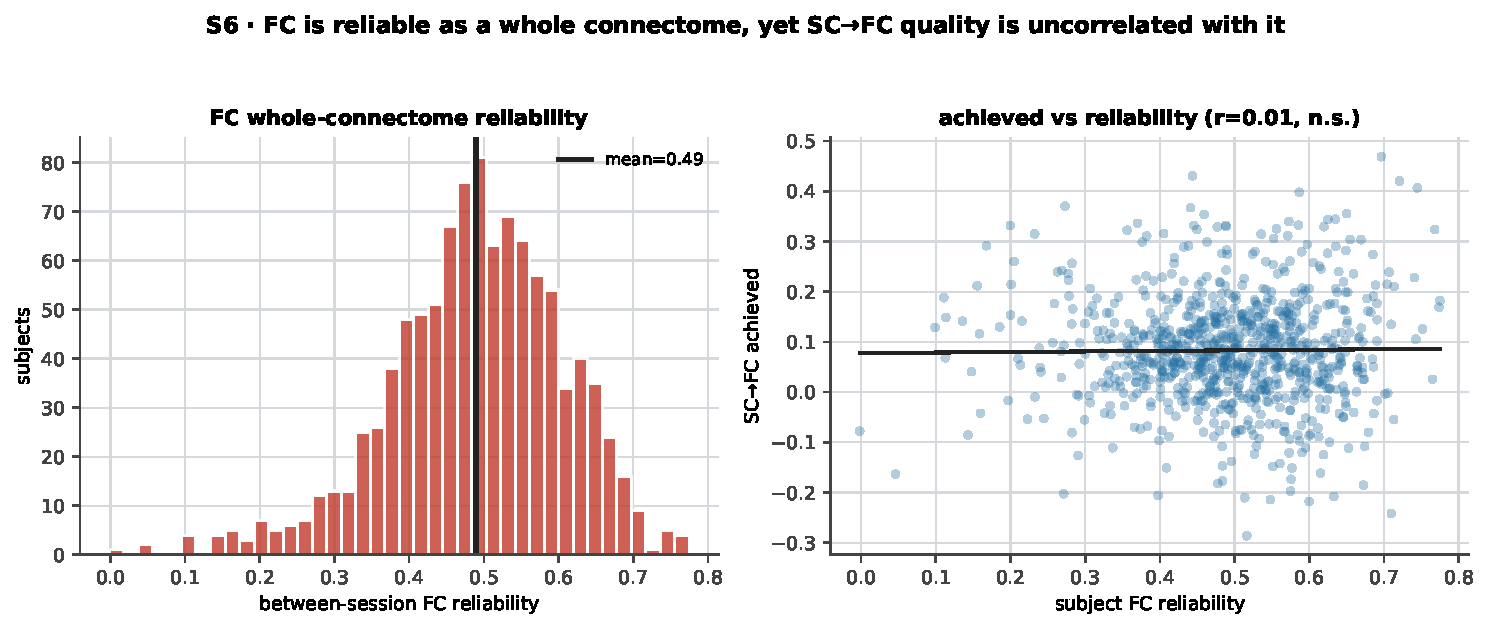
\includegraphics[width=0.9\linewidth]{S6_fc_reliability.pdf}
  \caption{FC reliability is reliable in aggregate, yet \scfc{} achieved quality is
  uncorrelated with per-subject FC reliability ($r=0.01$).}
\end{figure}

\noindent\emph{Source:} \texttt{sanity\_checks/noise\_sanity\_check/}.

\FloatBarrier
\section{Nonlinear Model Class}

\textbf{Concern.} The ceiling might be a linear-model failure.
\textbf{Design.} Swap estimators (HistGradientBoosting, KernelRidge-RBF) with representation
and splits held byte-identical. First, an estimator-trust check: a valid nonlinear probe must
preserve FC's known cognition lift.

\begin{table}[h]
\centering\small
\caption{Estimator trust check (FC $\rightarrow$ CogTotal). KernelRidge preserves FC's lift
and is the trustworthy probe; HGB destroys even FC's signal at $n\approx683$.}
\begin{tabular}{@{}lrrr@{}}
\toprule
\textbf{estimator} & \textbf{FC pearson} & \textbf{floor} & \textbf{FC lift} \\
\midrule
linear (BayesianRidge) & 0.451 & 0.372 & \textbf{+0.078} \\
KernelRidge & 0.338 & 0.282 & \textbf{+0.056} \\
HGB & 0.254 & 0.355 & $-$0.101 \\
\bottomrule
\end{tabular}
\end{table}

Under the trustworthy KernelRidge probe: (N1) no tractography representation clears the
\bvdemo{} floor (best $-0.029$); (N2) reconstruction $|\Delta|\le 0.0023$ vs linear and the
asymmetry ratio is unchanged (SC $1.62\times\!\to\!1.64\times$); (N3) bundle features add
nothing marginal over counts ($\Delta=-0.0049$). All decision rules return null --- the
findings are model-class robust.

\begin{figure}[h]
  \centering
  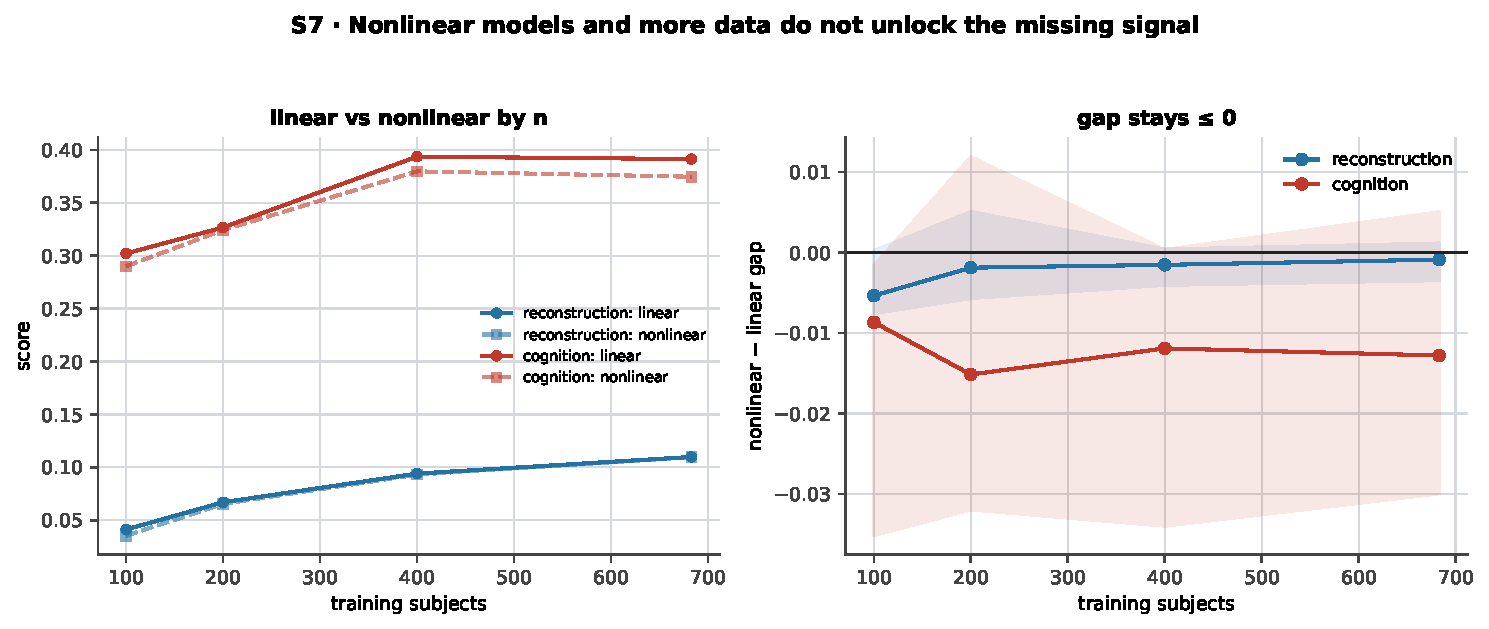
\includegraphics[width=0.9\linewidth]{S7_nonlinear_scaling.pdf}
  \caption{Linear vs nonlinear scores (left) and the nonlinear$-$linear gap vs sample size
  (right); the gap never grows into positive territory.}
\end{figure}

\noindent\emph{Source:} \texttt{non-linear-sanity-check/} (N1--N3).

\FloatBarrier
\section{Residual-Boost and Multimodal Sink}

\textbf{Concern.} Maybe the linear model used up the easy variance and a nonlinear model
tasked with the \emph{residual} would find structure.
\textbf{Design.} Hand the nonlinear model the out-of-fold linear prediction for free (no
leakage) and score only the improvement above it (N4 single-modality; N5 a multimodal sink
\texttt{[FC$\|$SC$\|$r2t$\|$bv$\|$demo]} that can exploit cross-modal conjunctions).

\begin{table}[h]
\centering\small
\caption{N4 reconstruction: a genuine but trivial nonlinear residual (every direction
$p=0.001$, but $\Delta\approx+0.005$, $\sim$4$\times$ below the +0.02 ``matters'' threshold).}
\begin{tabular}{@{}lrrrr@{}}
\toprule
\textbf{direction} & \textbf{template} & \textbf{final} & \textbf{$\Delta$} & \textbf{p} \\
\midrule
\fcsc & 0.1355 & 0.1405 & +0.0052 & 0.001 \\
\scfc & 0.0847 & 0.0866 & +0.0023 & 0.001 \\
FC$\rightarrow$r2t & 0.1113 & 0.1169 & +0.0058 & 0.001 \\
r2t$\rightarrow$FC & 0.0493 & 0.0526 & +0.0041 & 0.001 \\
\bottomrule
\end{tabular}
\end{table}

\begin{table}[h]
\centering\small
\caption{N5 cognition: combining modalities \emph{dilutes} FC; the cross-modal nonlinear
residual does not help. FC alone is the best predictor.}
\begin{tabular}{@{}lrrrr@{}}
\toprule
\textbf{target} & \textbf{bv+demo floor} & \textbf{FC alone} & \textbf{sink linear} & \textbf{sink residual} \\
\midrule
CogTotal & 0.373 & \textbf{0.436} & 0.401 & 0.381 \\
CogFluid & 0.298 & \textbf{0.306} & 0.301 & 0.286 \\
CogCrystal & 0.349 & \textbf{0.452} & 0.414 & 0.415 \\
\bottomrule
\end{tabular}
\end{table}

Cognition is comprehensively null (single-modality and cross-modal); reconstruction shows one
tiny real sliver that washes out under the sink ($-0.0023$, $p=0.935$). A clean null from an
OOF residual-boost means $y-\hat{y}_{\text{linear}}$ is noise with respect to the source ---
there is no learnable structure left at this $n$.

\noindent\emph{Source:} \texttt{non-linear-sanity-check/} (N4--N5).

\FloatBarrier
\section{Sample-Size Scaling}

\textbf{Concern.} The linear ceiling might be a sample-size ceiling.
\textbf{Design.} Learning curve at $n=100/200/400/{\sim}683$; does the nonlinear gap grow with
$n$?

\begin{table}[h]
\centering\small
\caption{Cognition (CogTotal): the nonlinear$-$linear gap is $\le 0$ at every $n$
(Spearman $\rho=+0.05$, $p=0.77$ $\Rightarrow$ flat), while the linear score climbs.}
\begin{tabular}{@{}rrrrr@{}}
\toprule
\textbf{n} & \textbf{linear} & \textbf{final} & \textbf{gap} & \textbf{p(gap$>$0)} \\
\midrule
100 & 0.302 & 0.290 & $-$0.0087 & 1.00 \\
200 & 0.327 & 0.324 & $-$0.0152 & 0.99 \\
400 & 0.394 & 0.380 & $-$0.0119 & 0.999 \\
$\sim$683 & 0.391 & 0.375 & $-$0.0128 & 0.99 \\
\bottomrule
\end{tabular}
\end{table}

For reconstruction the gap is negative at every $n$ and merely creeps toward zero from below
(an overfitting penalty vanishing, not signal appearing). The null is now robust to four
independent axes: model class (S3), the residual head-start (S4), cross-modal interactions
(S4 sink), and sample size (S5). Tested to $n\approx683$; the data converges \emph{to} zero,
not above it.

\noindent\emph{Source:} \texttt{non-linear-sanity-check/} (N6).

\FloatBarrier
\section{Richer Structural Representations}

\textbf{Concern.} Parcellated streamline counts may be too crude; named-bundle tractography
(\texttt{r2t}) might recover the missing signal.

\begin{table}[h]
\centering\small
\caption{E1 --- predicting FC from each structural representation (median \dpear). Count-SC
beats bundle-r2t on every metric.}
\begin{tabular}{@{}lr@{}}
\toprule
\textbf{representation} & \textbf{demeaned\_pearson} \\
\midrule
SC (streamline counts) & \textbf{0.0847} \\
kitchen-sink [SC$\|$r2t$\|$bv$\|$demo] & 0.0942 \\
SC + r2t & 0.0791 \\
r2t (bundle) & 0.0493 \\
r2t\_corr (bundle-similarity) & 0.0362 \\
\bottomrule
\end{tabular}
\end{table}

\begin{table}[h]
\centering\small
\caption{E5 --- downstream cognition (CogCryst). FC is the only representation above the
\bvdemo{} floor; the \texttt{r2t}$\rightarrow$synthetic-FC substitution chain does not recover
FC's signal.}
\begin{tabular}{@{}lrr@{}}
\toprule
\textbf{representation} & \textbf{CogCryst pearson} & \textbf{lift over bv+demo} \\
\midrule
\textbf{FC} & \textbf{0.451} & \textbf{+0.105} \\
bv+demo (floor) & 0.346 & 0 \\
SC & 0.267 & $-$0.079 \\
r2t$\rightarrow$synthFC & 0.180 & $-$0.166 \\
r2t & 0.164 & $-$0.183 \\
SC + r2t & 0.160 & $-$0.187 \\
r2t\_corr & 0.103 & $-$0.243 \\
\bottomrule
\end{tabular}
\end{table}

The \fcsc{} asymmetry holds on all six metrics at $p=0.001$ (E2); bundle features add nothing
marginal over counts ($\Delta=-0.0013$, E3); and the family/dorsal-stream SC mode does not map
cleanly to any single bundle mode (best $|\rho|=0.32$, E4). Counts are a sufficient statistic.

\begin{figure}[h]
  \centering
  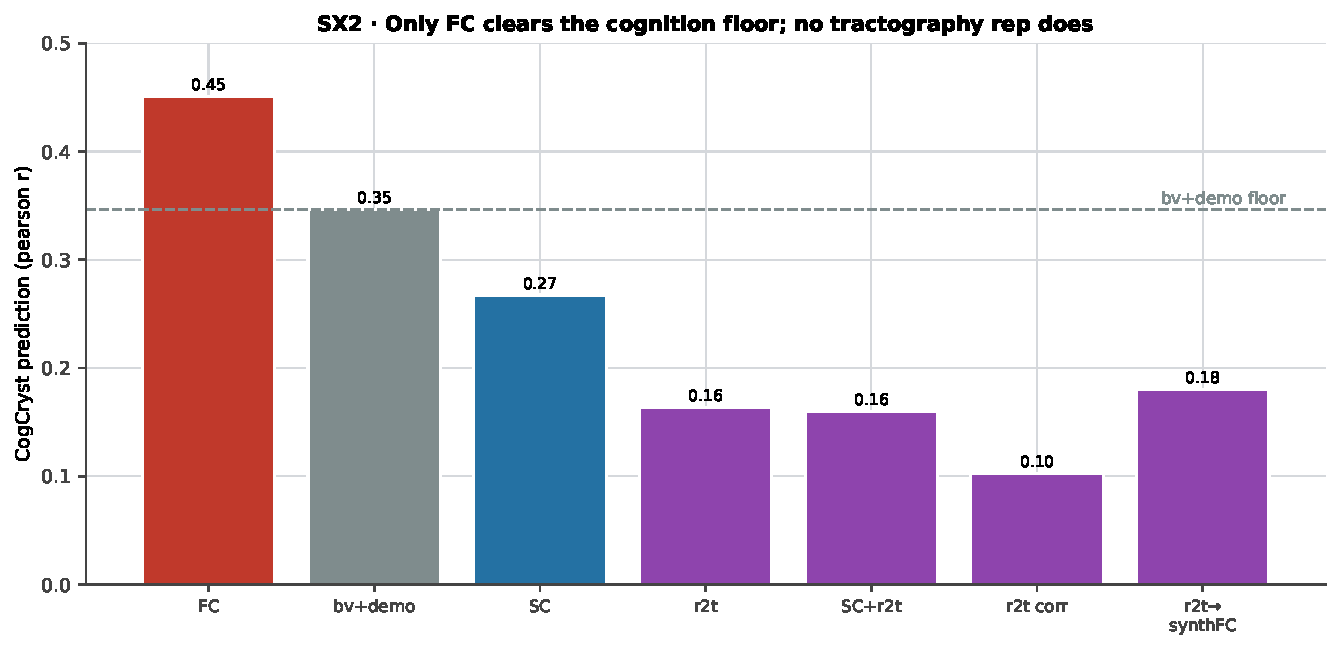
\includegraphics[width=0.85\linewidth]{SX2_tractography_downstream.pdf}
  \caption{Downstream cognition by representation: only FC clears the demographic floor.}
\end{figure}
\begin{figure}[h]
  \centering
  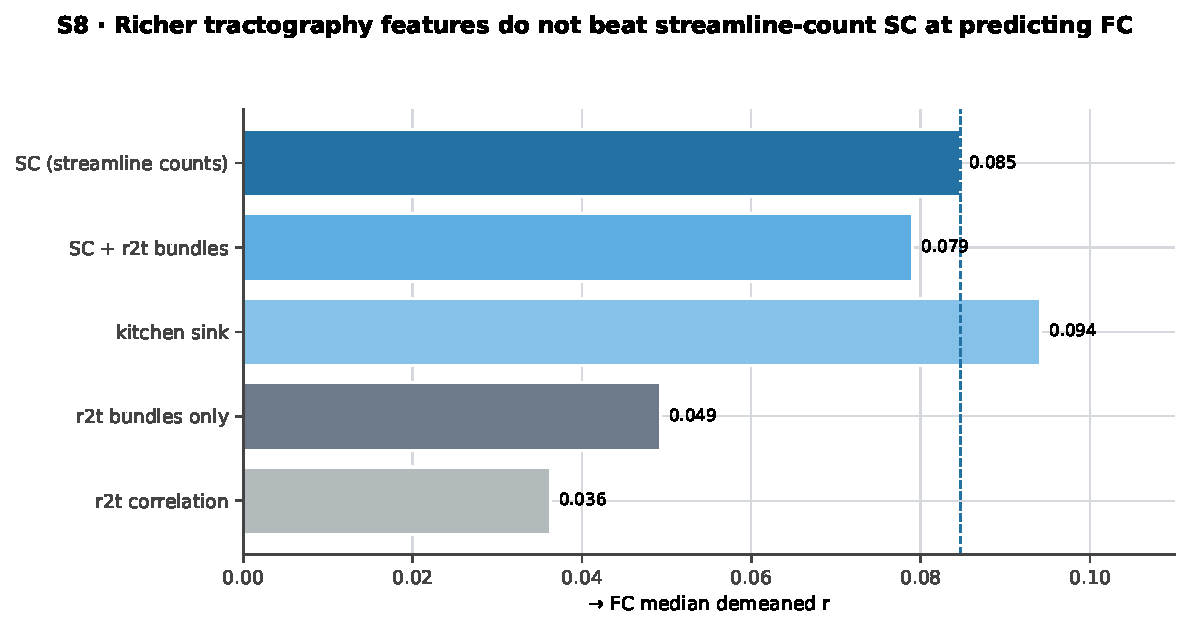
\includegraphics[width=0.7\linewidth]{S8_tractography.pdf}
  \caption{Predicting FC: richer tractography features do not beat streamline-count SC.}
\end{figure}

\noindent\emph{Source:} \texttt{tractography\_predict/} (E1--E5).

\FloatBarrier
\section{Mechanism-Mode Localization and Reliability Partialling}

\textbf{Framing.} The mechanism analysis is exploratory: the defensible claim is ``a
property-selected, low-variance, FC-predictable SC mode carries weak family signal,'' not
``PC3 is the mechanism.'' The component index migrates (PC3 in Glasser, PC4 in 4S456); effects
are small (FC$\rightarrow$PC $R^2\approx 0.22$--$0.24$; sibling AUC $\approx 0.58$). PC1 is a
sex/volume confound ($R^2\approx 0.89$--$0.93$) and is not a mechanism.

\textbf{Concern.} The visual / dorsal-attention localization could reflect higher tractography
reliability in posterior, short, high-strength connections.
\textbf{Design.} Partial edge strength and inter-region distance out of $|\text{PC3}|$
(together 41\% of its magnitude variance) and recompute Yeo-7 network enrichment.

\begin{table}[h]
\centering\small
\caption{Localization survives reliability partialling; visual--visual \emph{intensifies}.}
\begin{tabular}{@{}lrrr@{}}
\toprule
\textbf{network pair} & \textbf{raw enrichment} & \textbf{residualized} & \textbf{$\Delta$} \\
\midrule
visual $\|$ visual & 11.97$\times$ & \textbf{13.32$\times$} & +1.35 \\
dorsal attention $\|$ dorsal attention & 7.73$\times$ & \textbf{5.73$\times$} & $-$2.00 \\
dorsal attention $\|$ visual & 4.49$\times$ & \textbf{4.99$\times$} & +0.50 \\
\bottomrule
\end{tabular}
\end{table}

An independent FC scan-rescan cross-check adds nothing beyond the strength+distance proxy
(joint $R^2$ 41.2\% vs 41.0\%) and yields identical partialled localization. \emph{Honest
caveat:} this uses a strength+distance+FC-reliability proxy, not a gold-standard per-edge SC
ICC (which needs the HCP retest dMRI release); the 41\% $R^2$ is reported, not buried ---
reliability matters, and the surviving signal is the other half.

\begin{figure}[h]
  \centering
  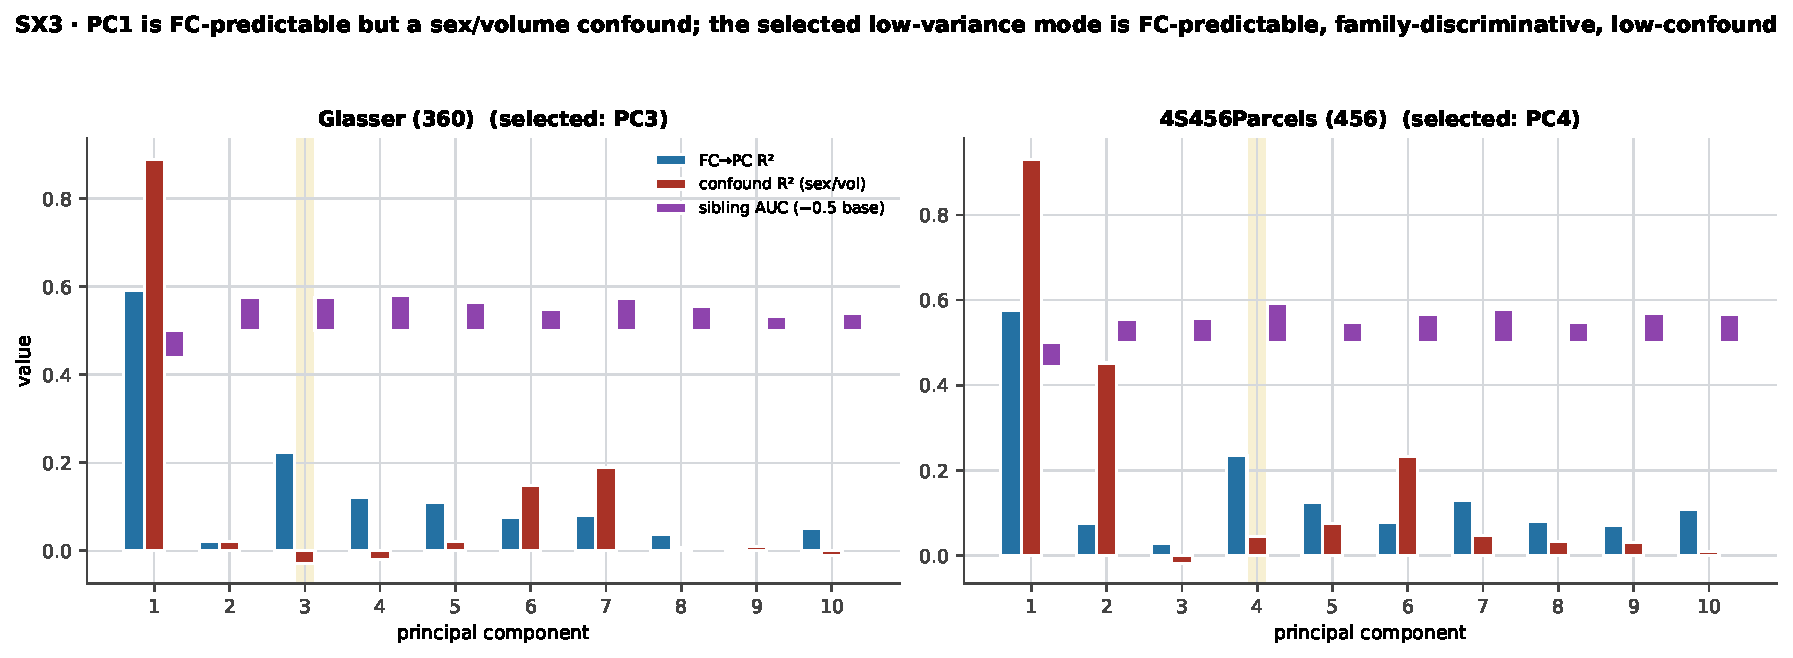
\includegraphics[width=\linewidth]{SX3_per_pc_confound.pdf}
  \caption{Per-PC FC-predictability, sex/volume confound, and sibling AUC. PC1 is
  FC-predictable but a confound; the selected low-variance mode is FC-predictable,
  family-discriminative, and low-confound.}
\end{figure}
\begin{figure}[h]
  \centering
  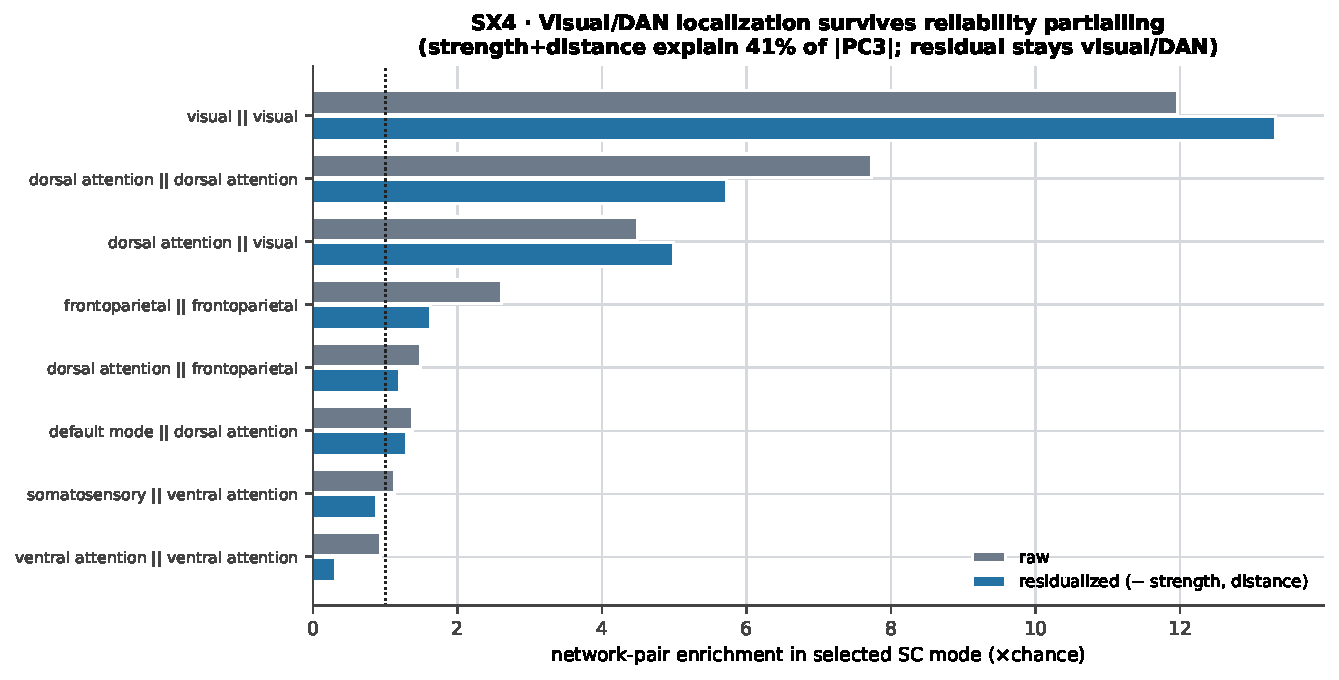
\includegraphics[width=0.85\linewidth]{SX4_pc_enrichment_partialled.pdf}
  \caption{Network-pair enrichment of the selected SC mode, raw vs reliability-residualized.}
\end{figure}

\noindent\emph{Source:} \texttt{sanity\_checks/tract\_check/},
\texttt{reproduction/family\_mechanism/outputs/f8\_*.csv}.

\FloatBarrier
\section{Completeness, Leak Guardrails, and Reproducibility}

The spine grid contains \textbf{13{,}640 cells} (2{,}640 reconstruction + 11{,}000
downstream); the merged output is complete (13{,}640/13{,}640), with zero non-finite values in
load-bearing metrics and zero hard leak failures.

\begin{table}[h]
\centering\small
\caption{Leak verdicts separate expected biological signal from implementation leakage.}
\begin{tabular}{@{}llr@{}}
\toprule
\textbf{Verdict} & \textbf{Meaning} & \textbf{Count} \\
\midrule
\texttt{ok} & no threshold violation & 3{,}344 \\
\texttt{EXPECTED\_SIGNAL} & raw connectome predicts sex/age (biological) & 4 \\
\texttt{EXEMPT\_FLAGGED} & input contains \bvdemo; sex/age expected & 1{,}052 \\
\texttt{LEAK\_FAIL} & non-exempt derived input exceeds threshold & \textbf{0} \\
\bottomrule
\end{tabular}
\end{table}

\textbf{Estimator-reporting rule.} Reconstruction leads with \dpear{} (raw Pearson is
dominated by the population-mean connectome); downstream scalar targets use BayesianRidge. A
resolved discrepancy showed PCA$\rightarrow$PLS scalar rows are ill-conditioned (e.g.\ Glasser
SC$\rightarrow$SC oracle \dpear{} 0.376 under PCA$\rightarrow$PLS vs 0.648 under BayesianRidge),
so every reported number names its estimator. \textbf{CSV outputs are the source of truth; W\&B
is a replay layer, not a dependency.} Family/mechanism ports are validated against the
notebooks with exact or near-exact regression tests.

\begin{figure}[h]
  \centering
  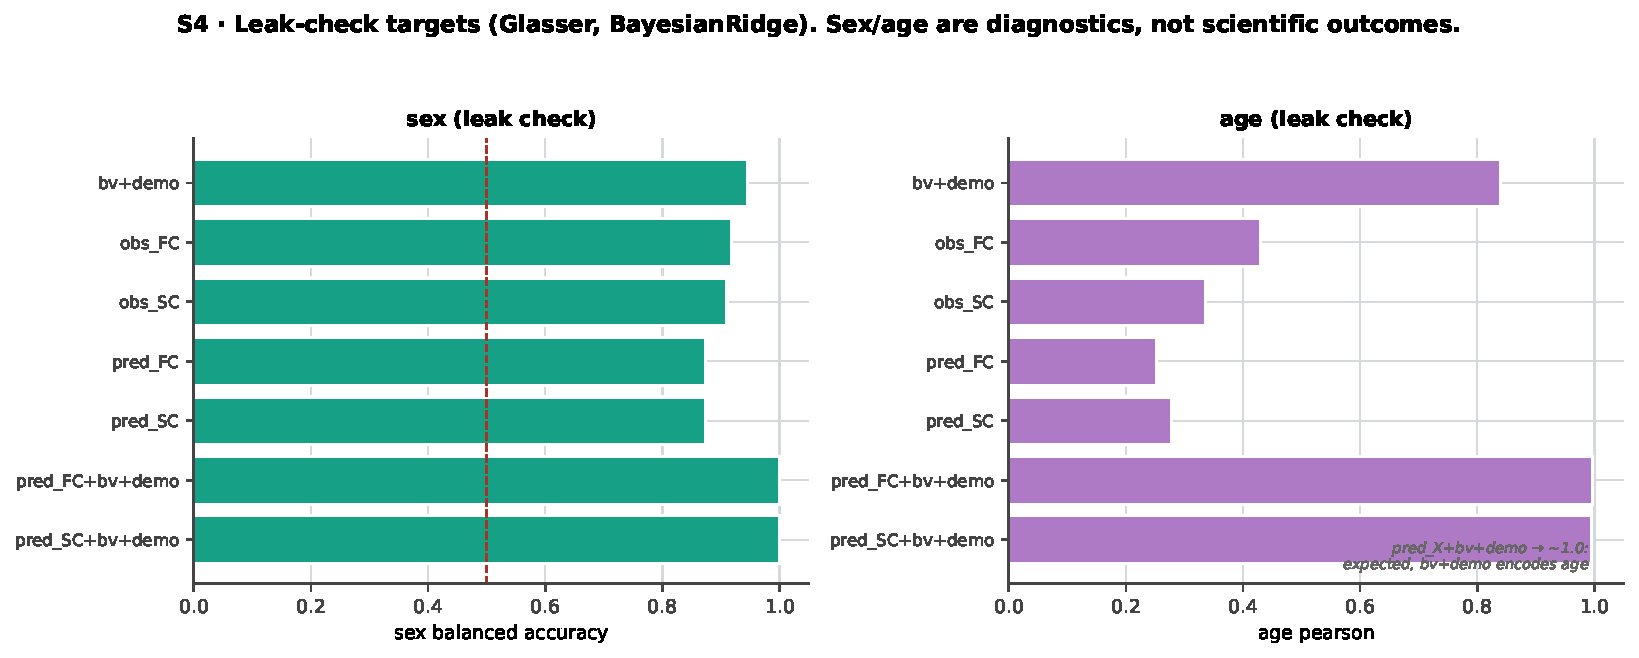
\includegraphics[width=\linewidth]{S4_leak_checks.pdf}
  \caption{Sex and age prediction by input (Glasser). These are diagnostics, not scientific
  outcomes; \texttt{pred\_X+bv+demo} reaching $\sim$1.0 for age is expected because
  \bvdemo{} encodes age.}
\end{figure}

\FloatBarrier
\section*{Summary --- every escape route, closed}
\addcontentsline{toc}{section}{Summary}

\begin{table}[h]
\centering\small
\caption{Each mundane explanation for the directional / negative results, and the check that
closes it.}
\begin{tabular}{@{}p{0.46\linewidth} c p{0.40\linewidth}@{}}
\toprule
\textbf{Mundane explanation} & \textbf{\S} & \textbf{Outcome} \\
\midrule
The asymmetry is a PCA reduction artifact & S1 & ratio $>1$ for raw-PLS, PCA, 3 JL; $p\le 0.001$ \\
\scfc{} fails because FC is noisy & S2 & \scfc{} reaches 17\% of FC ceiling; per-subject $r=0.01$ \\
A bigger / nonlinear model would find it & S3 & KernelRidge (validated on FC) finds nothing \\
The linear model left residual signal unused & S4 & OOF residual-boost null; +0.005 recon sliver washes out \\
More subjects would unlock it & S5 & nonlinear gap flat/$\le0$ from $n{=}100$ to $n{\approx}683$ \\
Streamline counts are too crude & S6 & r2t predicts FC worse, no marginal or cognition gain \\
The family mode is a reliability artifact & S7 & survives strength+distance+reliability partial (41\% $R^2$) \\
The grid is silently incomplete or leaking & S8 & 13{,}640/13{,}640 cells, 0 non-finite, 0 \texttt{LEAK\_FAIL} \\
\bottomrule
\end{tabular}
\end{table}

\noindent
\textbf{Narrowed, defensible claim.} In healthy young adults, under cross-sectional
normal-range cognition, the missing structural utility is not recovered by obvious changes in
dimensionality reduction, model class, structural representation, or sample size --- and the
\scfc{} shortfall is not an FC-noise artifact. The remaining open piece is SC's own
reliability, which is data-blocked pending test-retest dMRI.

\end{document}
